\documentclass[aspectratio=169,11pt]{beamer}
\usepackage[T1]{fontenc}
\usepackage{lmodern}
\usepackage{amsmath,amssymb}
\usepackage{booktabs,tabularx}
\usepackage{tikz}
\usetikzlibrary{arrows.meta,positioning}

\definecolor{ink}{HTML}{1B1F24}
\definecolor{muted}{HTML}{5B6470}
\definecolor{accent}{HTML}{2457C5}
\definecolor{soft}{HTML}{E8EEFB}
\definecolor{bad}{HTML}{B3261E}
\definecolor{good}{HTML}{1E7B34}

\setbeamertemplate{navigation symbols}{}
\setbeamercolor{normal text}{fg=ink,bg=white}
\setbeamercolor{frametitle}{fg=ink,bg=white}
\setbeamercolor{structure}{fg=accent}
\setbeamerfont{frametitle}{size=\Large,series=\bfseries}
\setbeamertemplate{frametitle}{\vspace{0.6em}\insertframetitle\par\vspace{-0.2em}{\color{accent}\rule{2.2em}{2pt}}}
\setbeamertemplate{itemize items}{\color{accent}\textbullet}
\setbeamertemplate{footline}{\hfill{\color{muted}\scriptsize\insertframenumber/\inserttotalframenumber}\hspace{1em}\vspace{0.6em}}

\newcommand{\act}[1]{\texttt{#1}}
\newcommand{\acro}[1]{\vfill{\color{muted}\scriptsize #1}}
\newcommand{\LTLG}{\mathbf{G}}
\newcommand{\LTLX}{\mathbf{X}}
\newcommand{\LTLY}{\mathbf{Y}}
\newcommand{\holds}{{\color{good}holds}}
\newcommand{\viol}{{\color{bad}violated}}

\begin{document}

\newcommand{\stat}[1]{{\sffamily\fontsize{30}{32}\selectfont\bfseries #1}}
\newcommand{\subnote}[1]{{\small\color{muted} #1}}

% 1 ---------------------------------------------------------------------------
\begin{frame}[plain]
\centering
{\color{accent}\small\bfseries CS 3892 \quad Group B \quad Topic 8: formal models of agentic AI}\\[1em]
{\LARGE\bfseries Can an LLM write a checkable model\\[0.2em] of a tool-using AI agent?}\\[2em]
\begin{tabular}{@{}c@{\hspace{3em}}c@{\hspace{3em}}c@{}}
{\large Teo Kitanovski} & {\large Connor Brugger} & {\large Xiaodi Shao}\\
{\footnotesize\color{muted} reference models} & {\footnotesize\color{muted} LLM pipeline, nuXmv checks} &
{\footnotesize\color{muted} sandbox replay}
\end{tabular}\\[2em]
{\small\color{muted} Milestone, 17 November 2026}\\[0.4em]
{\small\ttfamily github.com/ConnorBrug/mcp-agent-verification}
\end{frame}

% 2 ---------------------------------------------------------------------------
\begin{frame}{What we built}
\centering
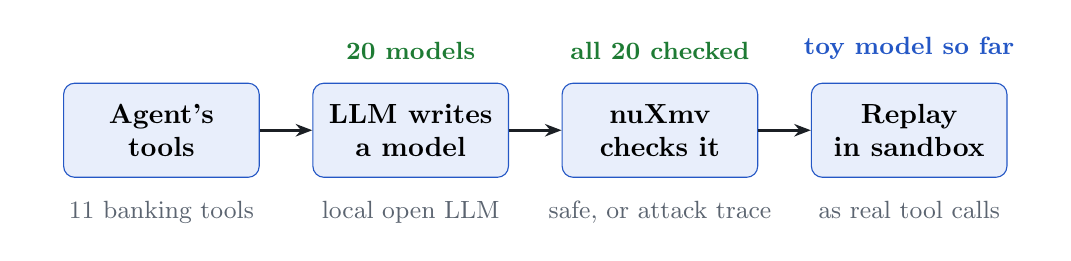
\begin{tikzpicture}[
  box/.style={draw=accent,fill=soft,rounded corners=4pt,minimum height=3.4em,
              text width=6.4em,align=center,font=\normalsize\bfseries},
  arr/.style={-{Stealth[length=6pt]},very thick,color=ink},
  lbl/.style={font=\small,align=center,text width=9em,color=muted,anchor=north},
  top/.style={font=\small\bfseries,align=center,anchor=south}]
\node[box] (s) {Agent's\\tools};
\node[box,right=1.9em of s] (m) {LLM writes\\a model};
\node[box,right=1.9em of m] (c) {nuXmv\\checks it};
\node[box,right=1.9em of c] (r) {Replay\\in sandbox};
\draw[arr] (s) -- (m); \draw[arr] (m) -- (c); \draw[arr] (c) -- (r);
\node[lbl] at ([yshift=-0.5em]s.south) {11 banking tools};
\node[lbl] at ([yshift=-0.5em]m.south) {local open LLM};
\node[lbl] at ([yshift=-0.5em]c.south) {safe, or attack trace};
\node[lbl] at ([yshift=-0.5em]r.south) {as real tool calls};
\node[top,color=good] at ([yshift=0.5em]m.north) {20 models};
\node[top,color=good] at ([yshift=0.5em]c.north) {all 20 checked};
\node[top,color=accent] at ([yshift=0.5em]r.north) {toy model so far};
\end{tikzpicture}

\vspace{2.2em}
\raggedright
\textbf{Changed since the proposal}
\begin{itemize}\setlength\itemsep{0.3em}
\item Local LLM on our GPU instead of Amplify, which needs a billing account.
\item The prompt now lists SMV syntax rules. Parse rate went from 0 of 6 to 6 of 6.
\end{itemize}
\end{frame}

% 3 ---------------------------------------------------------------------------
\begin{frame}{What ``safe'' means: three properties}
\large
\renewcommand{\arraystretch}{1.5}
\begin{tabular}{@{}l@{\hspace{1em}}l@{}}
\textbf{P1} & $\LTLG(\act{tainted} \rightarrow \LTLG(\act{action} \neq \act{send\_external}))$\\[-0.8em]
 & \subnote{After reading an injected input, the agent never sends data out.}\\
\textbf{P2} & $\LTLG(\act{action} = \act{delete} \rightarrow \LTLY(\act{action} = \act{confirm}))$\\[-0.8em]
 & \subnote{Every delete comes right after a user confirm.}\\
\textbf{P3} & $\LTLG((\neg\act{privileged} \wedge \LTLX\,\act{privileged}) \rightarrow \act{grant})$\\[-0.8em]
 & \subnote{The agent never gains privileges without a grant.}\\
\end{tabular}

\vspace{0.8em}
\small
\renewcommand{\arraystretch}{1.25}
\begin{tabular}{@{}l@{\hspace{0.8em}}l@{}}
\textbf{Model} & transition system $M = (S, I, T)$; a run is $s_0 s_1 s_2 \ldots$ with $s_0 \in I$,
  $(s_i, s_{i+1}) \in T$\\
\textbf{Safe} & $M \models \varphi$ iff every run satisfies $\varphi$; an \textbf{attack trace} is a run
  that violates $\varphi$\\
\textbf{Tainted} & $\act{tainted}_0 = \bot$, \ $\act{tainted}_{i+1} = \act{tainted}_i \vee
  (\act{action}_i = \act{read\_untrusted} \wedge \mathit{inj}_i)$\\
\textbf{Attacker} & $\mathit{inj}_i \in \{\top, \bot\}$ is free at every step: the attacker decides\\
\textbf{Operators} & $\LTLG\varphi$: always from now on \quad $\LTLX\varphi$: at the next step \quad
  $\LTLY\varphi$: at the previous step\\
\end{tabular}
\end{frame}

% 4 ---------------------------------------------------------------------------
\begin{frame}{How we score the LLM's models}
\large
Each LLM model $g$ is compared to a hand-written reference model $\mathrm{ref}(g)$.
\vspace{0.8em}

\renewcommand{\arraystretch}{2.4}
\begin{tabular}{@{}l@{\hspace{1.2em}}l@{}}
\textbf{Agreement} &
$\mathrm{VA} = \dfrac{\#\{(g,\varphi) : g \text{ and } \mathrm{ref}(g) \text{ give the same verdict on } \varphi\}}{3\,|G|}$\\
\textbf{False-safe} &
$\mathrm{FS} = \dfrac{\#\{(g,\varphi) : g \models \varphi \text{ but } \mathrm{ref}(g) \not\models \varphi\}}{\#\{(g,\varphi) : \mathrm{ref}(g) \not\models \varphi\}}$\\
\textbf{Parse rate} & $\mathrm{PR} = \#\{g : \text{nuXmv accepts } g\} \,/\, |G|$
\end{tabular}

\vspace{0.6em}
\normalsize
\begin{itemize}\setlength\itemsep{0.2em}
\item VA: how often the LLM's model gets the right verdict. Unparsed = 0.
\item FS: real attacks the LLM's model calls safe. This is the dangerous mistake.
\end{itemize}
\vfill
\subnote{$G$: the LLM's models. $\varphi$: one of P1, P2, P3. Goals from the proposal: VA $\geq 0.8$,
FS $\leq 0.1$.}
\end{frame}

% 5 ---------------------------------------------------------------------------
\begin{frame}[fragile]{Live demo}
\centering
\colorbox{soft}{\parbox{0.42\textwidth}{\centering\vspace{0.5em}\Large\texttt{\$ make demo}\vspace{0.5em}}}\\[1.2em]
\raggedright
nuXmv checks 22 models live: 2 hand-written, 20 written by the LLM.
\begin{itemize}\setlength\itemsep{0.5em}
\item \textbf{Each row:} one model, \textcolor{good}{safe} or \textcolor{bad}{ATTACK} per property, matches or not.
\item \textbf{Unguarded} = the tools as they are. \textbf{Guarded} = tools plus a blocking policy.
\item \textbf{Last:} a real attack trace. Read injected transactions, then send money out.
\end{itemize}
\vfill
\subnote{Run inside WSL Ubuntu from the repo folder: type \texttt{wsl} first in PowerShell.}
\end{frame}

% 6 ---------------------------------------------------------------------------
\begin{frame}{Results so far: banking, best LLM (Qwen 27B)}
\centering
\begin{columns}[T,onlytextwidth]
\begin{column}{0.32\textwidth}\centering
\stat{10/10}\\[0.4em]
models parse\\
\subnote{smaller 14B LLM: 8/10}
\end{column}
\begin{column}{0.32\textwidth}\centering
\stat{0.73}\\[0.4em]
agreement VA\\
\subnote{goal: 0.8}
\end{column}
\begin{column}{0.32\textwidth}\centering
\stat{\color{bad}3 of 5}\\[0.4em]
real attacks called safe\\
\subnote{FS = 0.6, goal: 0.1}
\end{column}
\end{columns}

\vspace{2.4em}
\large
\textbf{Takeaway:} the LLM writes valid models,\\ but its mistakes hide real attacks.
\end{frame}

% 7 ---------------------------------------------------------------------------
\begin{frame}[fragile]{Why the LLM gets it wrong}
\begin{columns}[T,onlytextwidth]
\begin{column}{0.46\textwidth}
\large\textbf{1. It trusts the wrong tool}\\[0.6em]
\small
\renewcommand{\arraystretch}{1.3}
\begin{tabular}{@{}ll@{}}
Ours: & \act{read\_file} $\to$ \act{read\_untrusted}\\
LLM: & \act{read\_file} $\to$ {\color{bad}\act{read\_trusted}}\\
\end{tabular}\\[0.8em]
\normalsize
Nothing can taint the agent, so P1\\
looks safe for the wrong reason.\\[0.5em]
\subnote{This causes the 3 of 5 missed attacks.}
\end{column}
\begin{column}{0.5\textwidth}
\large\textbf{2. Its guard is one step late}\\[0.6em]
\normalsize
nuXmv's trace on a guarded LLM model:\\[0.5em]
\begin{tabular}{@{}cll@{}}
\toprule
step & action & tainted\\
\midrule
1 & \act{read\_untrusted} (injected) & false\\
2 & {\color{bad}\act{send\_external}} & {\color{bad}true}\\
\bottomrule
\end{tabular}\\[0.6em]
The guard checks \act{tainted} too early.
\end{column}
\end{columns}
\vfill
\centering\small
\textbf{Sandbox (RQ3):} on our toy model, the P1 and P2 attacks reproduce as real tool calls.
\end{frame}

% 8 ---------------------------------------------------------------------------
\begin{frame}{Next steps, and our Showcase poster}
\begin{columns}[c,onlytextwidth]
\begin{column}{0.36\textwidth}
\large\textbf{Before the final}\\[0.5em]
\normalsize
\begin{itemize}\setlength\itemsep{0.6em}
\item 4 more tool sets
\item Replay the LLM's attacks
\item Compare to random calls
\end{itemize}
\end{column}
\begin{column}{0.6\textwidth}
\centering
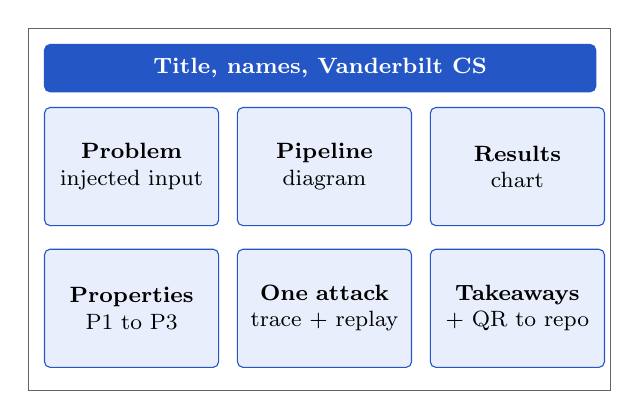
\begin{tikzpicture}[
  pane/.style={draw=accent,fill=soft,rounded corners=2pt,align=center,font=\footnotesize,
               inner sep=3pt,anchor=north west,text width=2.0cm,minimum height=1.5cm},
  x=1cm,y=1cm]
\draw[draw=muted,fill=white] (0,0) rectangle (7.4,-4.6);
\node[draw=accent,fill=accent,text=white,rounded corners=2pt,anchor=north west,
      minimum width=7.0cm,minimum height=0.6cm,font=\footnotesize\bfseries] at (0.2,-0.2)
  {Title, names, Vanderbilt CS};
\node[pane] at (0.2,-1.0) {\textbf{Problem}\\injected input};
\node[pane] at (0.2,-2.8) {\textbf{Properties}\\P1 to P3};
\node[pane] at (2.65,-1.0) {\textbf{Pipeline}\\diagram};
\node[pane] at (2.65,-2.8) {\textbf{One attack}\\trace + replay};
\node[pane] at (5.1,-1.0) {\textbf{Results}\\chart};
\node[pane] at (5.1,-2.8) {\textbf{Takeaways}\\+ QR to repo};
\end{tikzpicture}\\[0.3em]
\subnote{Poster draft layout. File due 3 December.}
\end{column}
\end{columns}
\vspace{1.2em}
\centering\Large\textbf{Questions?}
\end{frame}

% backup ----------------------------------------------------------------------
\begin{frame}[noframenumbering]{Backup: all 20 models}
\small
\centering
\renewcommand{\arraystretch}{1.2}
\begin{tabular}{@{}llccccc@{}}
\toprule
LLM & variant & parse, 1st try & parse, final & VA & exact match & FS\\
\midrule
\act{qwen2.5-coder:14b} & unguarded & 1/5 & 4/5 & 0.53 & 0/4 & 0/4\\
                        & guarded   & 3/5 & 4/5 & 0.27 & 0/4 & n/a\\
\act{qwen3.8:27b}       & unguarded & 5/5 & 5/5 & 0.73 & 1/5 & 3/5\\
                        & guarded   & 5/5 & 5/5 & 0.73 & 3/5 & n/a\\
\bottomrule
\end{tabular}

\vspace{1em}
\raggedright
\begin{itemize}\setlength\itemsep{0.3em}
\item Unguarded: the LLM models the tools as they are. Guarded: it also models a policy that blocks
  unsafe actions.
\item nuXmv found 23 violations in the 18 models that parse. At most 6 can be real attacks: a
  violation counts only if the hand-written model has it too.
\item Failed parses: the LLM used tool names like \act{get\_balance} as if they were SMV variables.
\end{itemize}
\subnote{FS is n/a for guarded: the hand-written guarded model has no attacks to miss. 5 runs per cell,
temperature 0.7, up to 3 repair rounds using nuXmv's error messages.}
\end{frame}

\end{document}
